%\documentclass[12pt]{article}
\documentclass[aip,jcp,preprint,superscriptaddress,floatfix]{revtex4-1}
\usepackage{url,graphicx,tabularx,array,geometry,amsmath,listings}
\setlength{\parskip}{2ex} %--skip lines between paragraphs
\setlength{\parindent}{20pt} %--don't indent paragraphs

\usepackage[colorinlistoftodos,prependcaption,textsize=tiny]{todonotes} %--TODO notes

\setlength{\headheight}{-50pt}
\setlength{\textheight}{700pt}
\setlength{\textwidth}{500pt}
\setlength{\oddsidemargin}{-10pt}
\setlength{\footskip}{50pt}
\usepackage{graphicx}% Include figure files
\usepackage{bm}
\usepackage{hyperref}
\usepackage{amsmath}
\graphicspath{{./Figures/}}

%-- Commands for header
\renewcommand{\title}[1]{\textbf{\large{#1}}\\}
\renewcommand{\line}{\begin{tabularx}{\textwidth}{X>{\raggedleft}X}\hline\\\end{tabularx}\\[-0.5cm]}
\newcommand{\leftright}[2]{\begin{tabularx}{\textwidth}{X>{\raggedleft}X}#1%
& #2\\\end{tabularx}\\[-1cm]}

%-- Convenient shortcuts
\newcommand{\x}{\mathbf{x}}
\newcommand{\vel}{\mathbf{v}}

%\linespread{2} %-- Uncomment for Double Space
\begin{document}

\title{\center{Molecular Dynamics} }
\rule{\textwidth}{1pt}
\leftright{The Molecular Sciences Software Institute}{Eliseo Marin-Rimoldi and John D.~Chodera} %-- left and right positions in the header

\bigskip

\section{Introduction}

Your first assignment consisted on implementing a Monte Carlo (MC) simulation
for the Lennard-Jones (LJ) particle in the canonical ensemble. 
As part of this task,
you developed code that computed pair-wise energies and forces for this model, 
as well as functions that computed interaction energies between molecules,
the total system potential energy, and the atomic virial for the estimation of pressure.

The objective of the new task is to extend your code by including the
necessary functionality to simulate the NVT ensemble of configurations 
of the LJ model using the molecular dynamics (MD). You will be 
assigned to work in teams to develop this project. The team will
decide how is best to design the new code: What functionality should be shared
between the two methods? What should the library should look like? How can
we improve reusability and extensibility? What data
structures should be used? Which unit tests should be implemented?
The primary learning goal of this activity is to think about interoperability and teamwork.

In the following sections, the relevant equations of the MD 
method will be presented and reference data for validation will be provided.

\subsection{Molecular dynamics (MD) theory}

A very common technique to simulate equilibrium and nonequilibrium
properties is the molecular dynamics method. 
The objective of this method is to simulate the evolution of a model over time
by integrating the Newtonian equations of motion to 
extract dynamic and thermodynamic properties. Thermodynamic
averages should be identical to those obtained by MC sampling
due to the ergodic hypothesis, given that we use the same model at the
same conditions. In an MD simulation, we can get additional dynamical
properties that is inaccessible in an MC simulation, such diffusivities or 
viscosities. 

Given a conservative system (i.e. the Hamiltonian does not depend on time), 
we can write the Newtonian equations of motion in Cartesian coordinates
from Hamilton's
equations as

\begin{equation}
	\ddot{\mathbf{r}} = \frac{\mathbf{f}_i\left( \mathbf{r} \right) }{\textit{m}_i}
\end{equation}

Where $\mathbf{r}$ is the vector of Cartesian coordinates, $\mathbf{f}_i$ and
 $\textit{m}_i$ are the forces and the mass of each atom, respectively.
These are 3N second order differential equations, where N is the number 
of atoms in the system. There are various finite difference approaches to solve
such equations. The basic idea in all of them is to move 
across time using finite time steps $\delta t$ and thus generate new atomic
positions. A good integration scheme is one that conserves energy 
and momentum, minimizes force evaluations, is stable and accurate. 

Unlike Monte Carlo methods, molecular dynamics integrators require both the the potential energies and forces to be everywhere continuous in order to produce well-behaved dynamics and sampling.
Because the potential function you implemented for Monte Carlo simply used a cutoff, this requires we add an additional option to use a switching function to ensure force continuity:
\begin{eqnarray}
U_\mathrm{sw}(r) = U_{LJ}(r) \, S(r)
\end{eqnarray}
where $U_{LJ}(r)$ is the Lennard-Jones potential you implemented earlier, 
\begin{equation}
U(r) = 4 \epsilon \left[\left(\frac{\sigma}{r}\right)^{12} -\left(\frac{\sigma}{r}\right)^{6} \right] 
\end{equation}
and the switching function $S(r)$ is selected to have a value of unity for $r \in [0, r_\mathrm{sw}]$, smoothly interpolates between 1 and 0 for $r \in (r_\mathrm{sw}, r_\mathrm{cut})$, and is zero for $r \in [r_\mathrm{cut}, \infty)$, with continuous first and second derivatives everywhere.
One such switching function is the following suggested by Skeel~\cite{Skeel.SIAMJSciComput.31.1363.2009}:
\begin{eqnarray}
S(r) &=& \begin{cases}
1 & r \le r_\mathrm{sw} \\
\frac{(r_\mathrm{cut}^2 - r^2) (r_\mathrm{cut}^2 + 2 r^2 - 3 r_\mathrm{sw}^2)}{(r_\mathrm{cut}^2 - r_\mathrm{sw}^2)^3} & r_\mathrm{sw} < r < r_\mathrm{cut} \\
0 & r \ge r_\mathrm{cut}
\end{cases}
\end{eqnarray}
To compute the force on atom $i$, we use the chain rule:
\begin{eqnarray}
f(\textbf{r}_k) &=& - \nabla_{\textbf{r}_k} \sum_{i < j} U(r_{ij}) =  - \sum_{i < j} \nabla_{\textbf{r}_k} \left[ U_{LJ}(r_{ij}) \, S(r_{ij}) \right] \nonumber \\
&=& - \sum_{i \ne k} \left\{ [ \nabla_{\textbf{r}_k} U_{LJ}(r_{ik}) ] \, S(r_{ik}) + U_{LJ}(r_{ik}) \,  \nabla_{\textbf{r}_k} S(r_{ik}) \right\}
\end{eqnarray}
The component derivatives are simply given by
\begin{eqnarray}
\nabla_{\mathbf{r}_k} U_{LJ}(r_{ik}) &=& \left. \frac{\partial U_{LJ}(r)}{\partial r} \right|_{r_{ik}} \nabla_{\mathbf{r}_k} r_{ik}  \\
&=& 4 \epsilon \left[- 12 \sigma^{12} r_{ik}^{-13} + 6 \sigma^6 r_{ik}^{-7} \right] \nabla_{\mathbf{r}_k} || \mathbf{r}_k - \mathbf{r}_i ||_2  \\
&=& - \frac{48 \epsilon}{r_{ik}} \left[2 \left(\frac{\sigma}{r}\right)^{12} - \left(\frac{\sigma}{r}\right)^{6} \right] \left( \frac{1}{2}\right) \left[ \frac{\mathbf{r}_k - \mathbf{r}_i}{r_{ik}} \right] \\
&=& - \frac{24 \epsilon}{r_{ik}} \left[2 \left(\frac{\sigma}{r}\right)^{12} - \left(\frac{\sigma}{r}\right)^{6} \right]  \left[ \frac{\mathbf{r}_k - \mathbf{r}_i}{r_{ik}^2} \right]  \\
\end{eqnarray}
and
\begin{eqnarray}
\nabla_{\mathbf{r}_k} S(r_{ik}) &=& \left. \frac{\partial S(r)}{\partial r} \right|_{r_{ik}} \nabla_{\mathbf{r}_k} r_{ik}  \\
&=&\frac{(2 r_{ik}) (r_\mathrm{cut}^2 -4 r_{ik}^2 + 3 r_\mathrm{sw}^2)}{(r_\mathrm{cut}^2 - r_\mathrm{sw}^2)^3} \left( \frac{1}{2}\right) \left[ \frac{\mathbf{r}_k - \mathbf{r}_i}{r_{ik}} \right] \\
\end{eqnarray}

\section{Integrators for Langevin dynamics}

One particularly good and widely used method is the Velocity Verlet algorithm
which is an improvement on the original Verlet method (i.e. less memory
intensive). The equations of this method are

\begin{equation}
	r \left( t + \delta t \right) = r \left( t \right) + v \left( t \right) \delta t + \frac{f \left(t \right) }{2 m} \delta t ^2
\label{eq:verlet.position.update}
\end{equation}

\begin{equation}
	v \left( t + \delta t \right) = v \left( t \right) + \frac{f \left( t + \delta t \right) + f \left(t \right) }{2m} \delta t
\end{equation}

This algorithm can be implemented as follows

\begin{itemize}
	\item Given a system state (i.e. positions and velocities), 
		compute forces on each atom
	\item Update the positions using Equation \ref{eq:verlet.position.update}
	\item Do a partial update to the velocities using the current forces
		\begin{equation}
			v \leftarrow v + \frac{f}{2m} \delta t
		\end{equation}
	\item Compute new forces using the updated positions
	\item Complete the update of the velocities with the old forces
		\begin{equation}
			v \leftarrow v + \frac{f}{2m} \delta t
		\end{equation}

\end{itemize}

\subsection{Technical considerations}

%\textbf{Energy conservation. } The velocity verlet algorithm has very good
%energy conservation properties. It is always a good check to see if 
%there is no drift in energy during the course of the simulation.

\textbf{Choice of timestep.} 
Unlike Metropolis Monte Carlo, molecular dynamics methods do not sample exactly from the target equilibrium density $\pi(\x,\vel)$, but instead sample from a density $\rho_{\Delta t}(\x,\vel)$ that increasingly deviates from the target equilibrium density as the timestep $\Delta t$ increases (Figure~\ref{figure:timestep-dependent-error}).
Using a timestep that is too large will result in large errors in the sampled density $\rho_{\Delta t}(\x)$ or, worse yet, unstable dynamics that might cause the simulation to ``explode''  and rapidly accumulate NaNs.

Traditional guidelines suggest restricting your timestep to be no bigger than $\frac{1}{10}$ the fastest vibrational frequency in the system.
For a pair of Lennard-Jones particles separated by $r_\mathrm{min} = 2^{1/6} \sigma$ where their interaction is minimized, the vibrational period for small oscillations about the minimum is given by
\begin{eqnarray}
T &\approx& 2 \pi \sqrt{ \frac{\mu}{K} } 
\end{eqnarray}
Here, the effective spring constant $K = \left. \frac{\partial^2 U_{LJ}}{\partial r^2} \right|_{r_\mathrm{min}} = 72 \epsilon / r_\mathrm{min}^2$ and the effective mass $\mu = (m^{-1} + m^{-1})^{-1} = m/2$ give a period of 
\begin{eqnarray}
T \approx 2 \pi \sqrt{\frac{2^{1/3} m \sigma^2}{144 \epsilon}} \approx 0.09354 \sqrt{\frac{m \sigma^2}{\epsilon}}
\end{eqnarray}
suggesting we should use a maximum timestep of $\Delta t \le T/10$.
More detailed discussion of the timestep-induced error can be found in Leimkuhler and Matthews~\cite{LeimkuhlerMatthewsBook} and work that uses nonequilibrium approaches to quantify this error~\cite{VVVR}.

\begin{figure}[h]
\centering
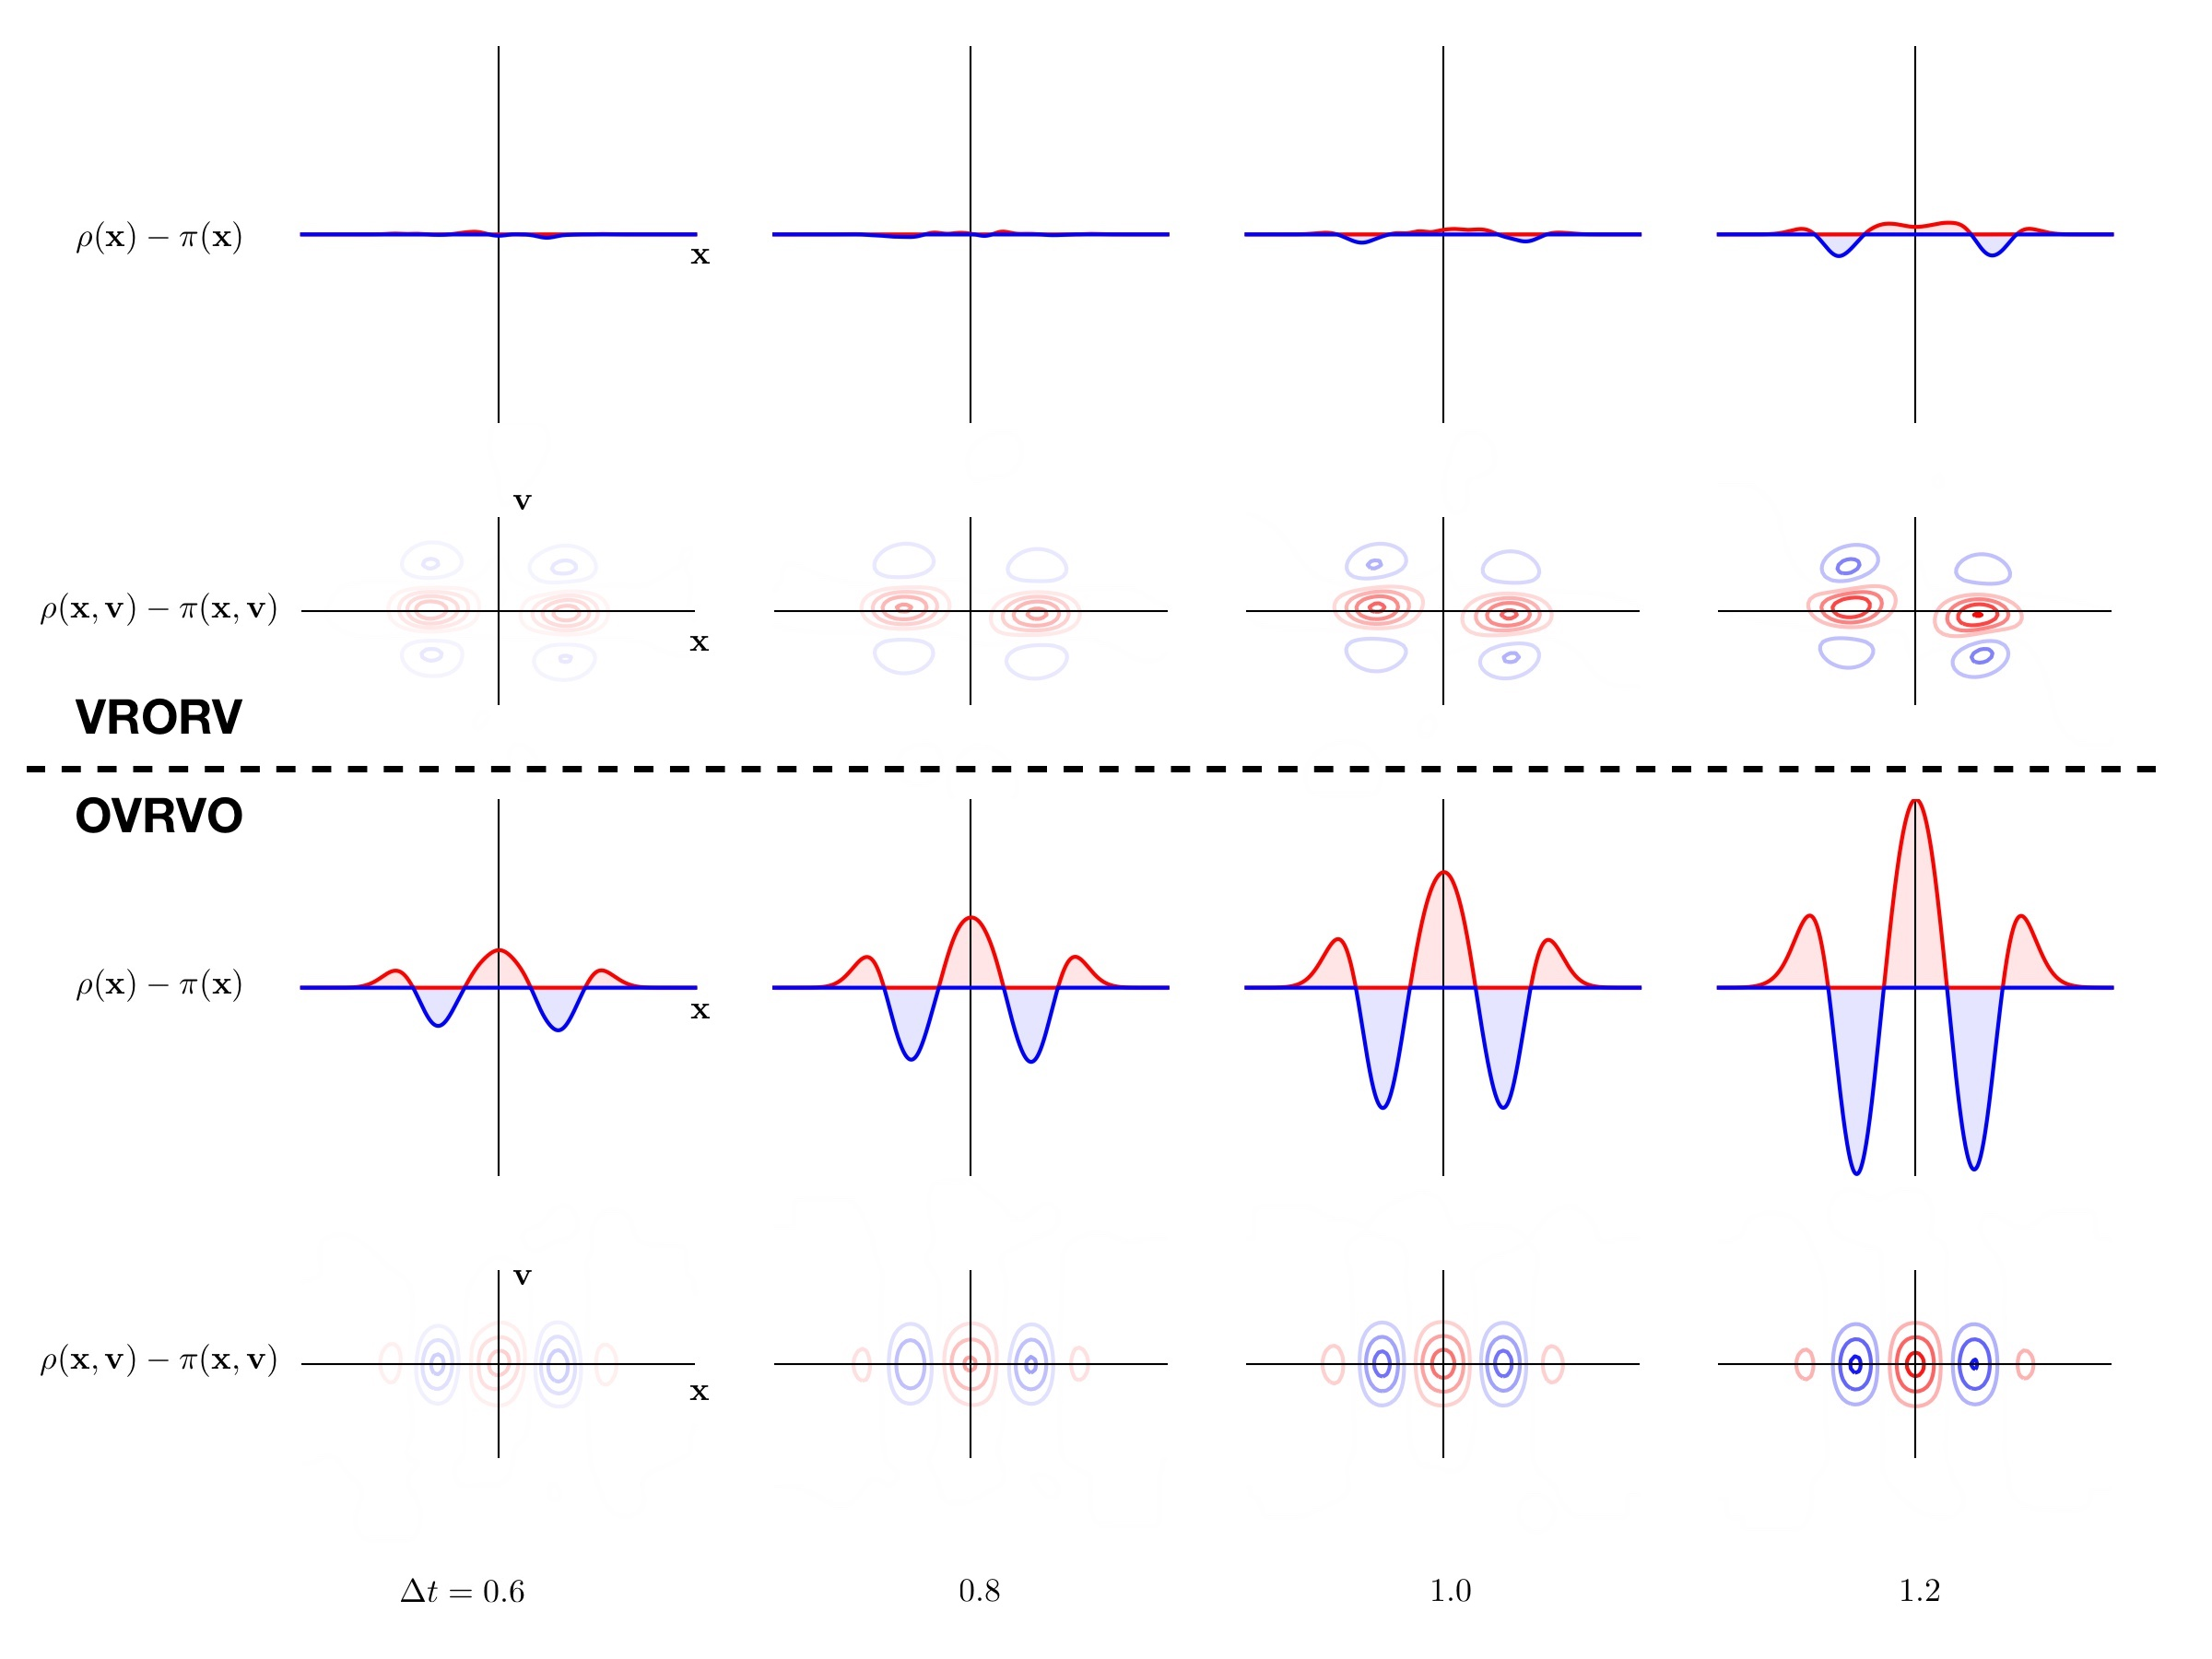
\includegraphics[width=1.0\textwidth]{figures/quartic_eq_joint_dist_array_w_x_marginals.jpg}

\caption{{\bf Different Langevin integrator splittings lead to different timestep-dependent errors in the sampled configuration and phase space densities.}
The quantity $\rho(\x,\vel) - \pi(\x,\vel)$ measures the deviation of the sampled phase space density $\rho_{\Delta t}(\x,\vel)$ from the target equilibrium density $\pi(\x,\vel)$ as a function of timestep for a quartic potential $U(x) = x^4$.
The marginal error in configuration space only, $\rho(\x) - \pi(\x)$, is the one-dimensional projection of this error.
Two different Langevin integrators derived from different Trotter splittings are shown: VRORV (also known as the BAOAB integrator by Leimkuhler and Matthews~\cite{gBAOAB,BAOAB}) and OVRVO (also known as VVVR~\cite{VVVR} or the integrator of Bussi and Parrinello~\cite{BussiParrinello}).
Integrators based on different splittings can lead to very different error properties in positions and velocities.
We recommend using VRORV if accurate sampling configurations is necessary (e.g.~for computing configurational properties) and OVRVO if accurate sampling of velocities is necessary (e.g.~for velocity correlation functions or kinetic properties).
\label{figure:timestep-dependent-error}
}
\end{figure}  

\textbf{Initial positions.} 
For molecular dynamics simulations, the main consideration is that the initial forces must not be so large that the system rapidly heats up and becomes numerically unstable.
Standard biomolecular systems must generally be subjected to energy minimization to produce forces small enough to run molecular dynamics, but several options are available for the simple Lennard-Jones system considered here.
While placing atoms randomly is more dangerous as core overlaps might exist, leading to huge repulsion forces, as in the Monte Carlo example, it is possible to use a crystalline lattice as an initial configuration, since this configuration will generally have relatively small forces. 
You could even first relax the system using the translation moves of your MC code, which only use energy differences forces for sampling and hence will not become numerically unstable due to large forces; a sampled configuration generated from your MC code could be used to initialize dynamics.

\textbf{Initial velocities.} 
Initial velocities can be generated from the Maxwell-Boltzmann distribution at the desired temperature
\begin{equation}
	\rho \left(\mathbf{v}_i\right) = \left( \frac{m_i}{2 \pi k_B T} \right)^{1/2} \exp \left[ - \frac{m_i \mathbf{v}_i^2 } {2 k_B T }  \right]
\end{equation}
This can be done by sampling the velocities for each particle from a Gaussian distribution
\begin{equation}
       \mathbf{v}_i \sim \mathcal{N}(0, \sigma_i^2)
\end{equation}
where the variance $\sigma_i^2$ is given by
\begin{equation}
	\sigma_v^2 = \frac{k_B T}{m_i}
\end{equation}

% JDC: We don't need to remove COM translational velocities for Langevin integrators.
%Once the velocities are assigned to the atoms, we must set the system momentum to zero to avoid any translational drift. 
%We do this by 
%\begin{itemize}
%	\item Find the net momentum of the system $\mathbf{P} = \sum m_i \mathbf{v}_i$
%	\item Reassign initial atomic velocities as
%		\begin{equation}
%			\mathbf{v}_i \leftarrow \mathbf{v}_i - \frac{\mathbf{P}} { N m_i}
%		\end{equation}
%\end{itemize}

\textbf{Long-range dispersion correction.}
Because a switch function is now employed, we must use a modified form of the long-range dispersion correction that accounts for the switching off of the potential over $r \in [r_\mathrm{sw}, r_\mathrm{cut}]$.
The simplest way to implement this is to numerically compute the long-range correction via
\begin{eqnarray}
U_\mathrm{tail} &=& N \frac{N}{V} \int_{r_\mathrm{sw}}^\infty 4 \pi r^2 \, dr \, U_{LJ}(r) [1 - S(r)] 
\end{eqnarray}
where the integral is performed using numerical quadrature, such as the \href{https://docs.scipy.org/doc/scipy/reference/generated/scipy.integrate.quad.html}{\tt scipy.integrate.quad}, to some sufficiently large $r \sim 10 \sigma$.

\textbf{Periodic boundary conditions and minimum image distance.} 
As in the MC case, your MD code should also implement these features.

\newpage
%
\bibliographystyle{aip.bst}
\bibliography{references.bib}

\end{document}
